\documentclass[twoside]{article}
\usepackage{amsmath,amsthm,amssymb,amsfonts,amscd}
\usepackage{url}
\usepackage{listings}
\usepackage{array}
\usepackage{lmodern}
\usepackage{authblk}
\usepackage[bookmarksnumbered, colorlinks, plainpages]{hyperref}
\usepackage{xcolor}
\usepackage{tikz}
\usetikzlibrary{shapes, arrows.meta, positioning}
\newtheorem{theorem}{Theorem}[section]
\newtheorem{lemma}[theorem]{Lemma}
\newtheorem{proposition}[theorem]{Proposition}
\newtheorem{corollary}[theorem]{Corollary}
\theoremstyle{definition}
\newtheorem{definition}[theorem]{Definition}
\newtheorem{example}[theorem]{Example}
\newtheorem{exercise}[theorem]{Exercise}
\newtheorem{conclusion}[theorem]{Conclusion}
\newtheorem{conjecture}[theorem]{Conjecture}
\newtheorem{criterion}[theorem]{Criterion}
\newtheorem{summary}[theorem]{Summary}
\newtheorem{axiom}[theorem]{Axiom}
\newtheorem{problem}[theorem]{Problem}
\theoremstyle{remark}
\newtheorem{remark}[theorem]{Remark}
\numberwithin{equation}{section}
\definecolor{codegray}{gray}{0.95}
\usepackage[english]{babel}
\usepackage{graphics}
\usepackage{epsfig}
\usepackage{graphicx}
\usepackage{float} %Coloca las imagenes justo en el lugar donde se desea con el
%comando \begin{figure}[H]
	\usepackage{subfigure} %permite agregar subfiguras
	\usepackage{epstopdf}
	%%%%%%%%%%%%%%%%%%%%%%%%%%%%%%%%%%%
	% Acentuación y símbolos en español
	%%%%%%%%%%%%%%%%%%%%%%%%%%%%%%%%%%%
	\usepackage[utf8x]{inputenc}
	%%%%%%%%%%%%%%%%%%%%%%%%%%%%%%%%%%%
	\usepackage{fancyhdr}
	\textwidth 35pc
	\textheight 47pc
	\oddsidemargin 1.5pc
	\evensidemargin 1.5pc
	\voffset -1pc
	\renewcommand{\thefootnote}{}
	\setcounter{page}{1} %*** # primera pagina***
	\fancypagestyle{plain}{\fancyhf{}%
		\fancyhead[L]{\footnotesize{Gravity as a VA/ET density gradient Vol. 2, No. 23 (2025), pp. \pageref{begin-art}--\pageref{end-art} \vspace{-6mm} 
		}}%
		\renewcommand{\headrulewidth}{0pt}\renewcommand{\footrulewidth}{0pt}}
	
	\fancypagestyle{headings}{\fancyhf{}%
		\renewcommand{\headrulewidth}{0.4pt}%
		\renewcommand{\footrulewidth}{0.4pt}%
		\fancyhead[LE,RO]{\thepage}%
		\fancyhead[RE]{Mohamed Makraini}%
		\fancyfoot[C]{\footnotesize{Gravity as a density gradient VA/ET Vol. 2, No. 23 (2025), pp. \pageref{begin-art}--\pageref{end-art}}}}
	
	
	%%%%%%%%%%%%%%%%%%%%%%%%%%%%%%%%%%
	% Declaraciones, nuevos comandos, etc.%
	%%%%%%%%%%%%%%%%%%%%%%%%%%%%%%%%%%
	\newtheorem{teo}{Teorema}[section]
	\newtheorem{propo}{Proposici\'on}[section]
	\newtheorem{lema}{Lema}[section]
	\newtheorem{corl}{Corolario}[section]
	\theoremstyle{definition}
	\newtheorem{defi}{Definici\'on}[section]
	\theoremstyle{example}
	\newtheorem{ejem}{Ejemplo}[section]
	\theoremstyle{remark}
	\newtheorem{nota}{Nota}[section]
	%%%%%%%%%%%%%%%%%%%%%%%%%%%%%%%%%%%%%%%
	% Enumeración de ecuaciones
	%%%%%%%%%%%%%%%%%%%%%%%%%%%%%%%%%%%%%%%
	\renewcommand{\theequation}{\thesection.\arabic{equation}}
	\numberwithin{equation}{section}%%%%%%%%%%%%%%%%%%%%%%%%%%%%%
	
	
	\begin{document}
		\label{begin-art}
		\pagestyle{headings}
		\thispagestyle{plain} 
		\footnote{\hspace{-18.1pt}\\ Corresponding author: Mohamed Makraini}
		\selectlanguage{english}
		\begin{center}
			{\LARGE\bfseries Standard Model: the Higgs mechanism as spontaneous symmetry breaking of the quantum vacuum. \par }
			
			\vspace{3mm}

			{\large Mohamed Makraini (\url{mk.makraini@mk4physics.eu})}\\
			Independent Researcher\\
			Málaga, Spain
			
		\end{center}
		

		
		\selectlanguage{english}
		
		\begin{abstract}

	We present a simulation of the coupling between the Higgs field (\( \Phi \)), the density of the Absolute Vacuum/Space-Time (\( \varrho \)), and an emergent curvature interpreted as gravitational. The model allows variation of key physical parameters.
	
	We argue that the Higgs field does not acquire mass via spontaneous symmetry breaking in the quantum vacuum~\cite{higgs1964}, but rather through direct interaction with the Absolute Vacuum, which lacks space-time structure. The resulting spacetime curvature emerges from AV flux effects, without invoking graviton exchange~\cite{rovelli2018}.



			
			\textbf{Keywords:} Absolute Vacuum, Higgs field, quantum density, emergent gravity, symmetry breaking.
		\end{abstract}
		
		
		\selectlanguage{english}
		
	\section{Introduction}
	
	The Higgs mechanism in the Standard Model postulates that particles acquire mass through spontaneous symmetry breaking in a scalar field \cite{higgs1964}. However, this work proposes an alternative paradigm in which mass emerges from a fundamental interaction with a pre-spacetime Absolute Vacuum (AV).\\
	
	\textbf{Advanced Simulation:} Higgs–Absolute Vacuum (AV) Equation with Adjustable Parameters\\
	\textbf{Objective:} To simulate the coupling between the Higgs field (\(\Phi\)), the AV/ST density (\(\varrho\)), and emergent gravity, by varying key physical parameters.\\
	
	\section{Modified Master Equation}
	
	We incorporate: 
	
	\begin{itemize}
	\item \textbf{Explicit dependence of the Higgs mass} (\(m_H\)) on \(\varrho\).
	\item \textbf{Gravitational coupling} (\(\kappa\)) as a dynamic variable.
	\item \textbf{AV flux} (\(\mathcal{F}_{\mu\nu}\)), analogous to a gauge field.
	\end{itemize}
	
	\textbf{Higgs Equation in AV/ST}: 
	
	\begin{equation}\label{e1}
		\left( \Box + \xi R + m_H^2(\varrho) + \kappa \mathcal{F}_{\mu\nu} \mathcal{F}^{\mu\nu} \right) \Phi = 0
	\end{equation}
	
	where:  
	- \(\xi R\): Coupling to curvature (Higgs-inflation type).\\
	- \(m_H^2(\varrho) = v^2 (1 - e^{-\varrho^2})\): Effective mass dependent on \(\varrho\).\\
	- \(\mathcal{F}_{\mu\nu} = \partial_\mu \mathcal{A}_\nu - \partial_\nu \mathcal{A}_\mu\): AV flux tensor.\\
	
	\subsection{Analysis Plan}
	
	\begin{itemize}
		\item Model A: Higgs with Spontaneous Symmetry Breaking (SSB)
		\item Model B: Higgs with Interaction with the Absolute Vacuum (AV)
		\item Physical and Mathematical Comparison
	\end{itemize}
	
		
	\subsection{MODEL A: Spontaneous Symmetry Breaking (SSB)}
	
	Lagrangian (with potential):
	
	\begin{equation}\label{e2}
		\mathcal{L}_{\text{SSB}} = \frac{1}{2} \partial^\mu \phi \, \partial_\mu \phi - V(\phi), \quad \text{with} \quad V(\phi) = -\frac{1}{2} \mu^2 \phi^2 + \frac{1}{4} \lambda \phi^4
	\end{equation}
	
	Euler–Lagrange equation:
	\begin{equation}\label{e3}
		\frac{d}{dt} \left( \frac{\partial \mathcal{L}}{\partial \dot{\phi}} \right) - \frac{\partial \mathcal{L}}{\partial \phi} = 0
	\end{equation}
	
	We compute:
	\begin{itemize}
		\item $\displaystyle \frac{\partial \mathcal{L}}{\partial \dot{\phi}} = \dot{\phi}$
		\item $\displaystyle \frac{d}{dt} ( \dot{\phi} ) = \ddot{\phi}$
		\item $\displaystyle \frac{\partial \mathcal{L}}{\partial \phi} = -\frac{dV}{d\phi} = \mu^2 \phi - \lambda \phi^3$
	\end{itemize}
	
	Result:
	\begin{equation}\label{e5}
		\boxed{ \ddot{\phi} + \mu^2 \phi - \lambda \phi^3 = 0 }
	\end{equation}
	
	This is the \textbf{classical Higgs model}, where:
	\begin{itemize}
		\item The Higgs mass is $ m_H^2 = 2\mu^2 $
		\item The solution stabilizes at $ \phi = v = \sqrt{\mu^2/\lambda} $
	\end{itemize}	       	
	
	\subsection{MODEL B: Interaction with the Absolute Vacuum (AV)}
	
	\textbf{Lagrangian:}
	
	\begin{equation}
		\mathcal{L}_{\text{AV}} = \frac{1}{2} \partial^\mu \phi \, \partial_\mu \phi - \frac{1}{2} m^2(\rho) \phi^2 - \frac{1}{2} \xi R \phi^2 - \frac{1}{2} \kappa \rho \phi^2
	\end{equation}
	
	\textbf{where:}
	\begin{equation}
		m^2(\rho) = v^2 \left( 1 - e^{-(\rho/\rho_c)^2} \right)
	\end{equation}
	
	As before, we apply Euler–Lagrange:
	
	\begin{itemize}
		\item $\displaystyle \frac{\partial \mathcal{L}}{\partial \dot{\phi}} = \dot{\phi} \quad \Rightarrow \quad \ddot{\phi}$
		\item $\displaystyle \frac{\partial \mathcal{L}}{\partial \phi} = \left[ m^2(\rho) + \xi R + \kappa \rho \right] \phi$
	\end{itemize}
	
	\textbf{Result:}
	\begin{equation}
		\boxed{
			\ddot{\phi} + \left[ m^2(\rho) + \xi R + \kappa \rho \right] \phi = 0
		}
	\end{equation}
	
	\renewcommand{\arraystretch}{1.5}
	\begin{table}[h]
		\centering
		\begin{tabular}{|>{\centering\arraybackslash}m{4.2cm}|m{5.5cm}|m{5.5cm}|}
			\hline
			\textbf{Feature} & \textbf{SSB Model} & \textbf{AV Model} \\
			\hline
			Potential &
			$-\frac{1}{2}\mu^2 \phi^2 + \frac{1}{4} \lambda \phi^4$ &
			No $\phi^4$; mass induced by AV \\
			\hline
			Equation of motion &
			$\ddot{\phi} + \mu^2 \phi - \lambda \phi^3 = 0$ &
			$\ddot{\phi} + [m^2(\rho) + \xi R + \kappa \rho] \phi = 0$ \\
			\hline
			Mass generation &
			From the shape of the potential (spontaneous) &
			From physical interaction with the AV \\
			\hline
			Equilibrium point &
			Fixed at $\phi = \pm v$ &
			Dynamic depending on $\rho(t)$ \\
			\hline
			Symmetry &
			Spontaneously broken &
			Preserved, but interaction defines behavior \\
			\hline
		\end{tabular}
		\caption{Comparison between the SSB Model (Spontaneous Symmetry Breaking) and the AV Model (Absolute Vacuum).}
		\label{tab:models}
	\end{table}
	
	\section{Extension of the Absolute Vacuum (AV) Lagrangian}
	
	\subsection{General Structure}
	
	The AV differs from the conventional quantum vacuum in that:
	\begin{itemize}
		\item It has no space-time structure \cite{rovelli2018}
		\item Its density (\(\varrho\)) is a fundamental parameter
		\item It produces non-local effects on quantum fields
	\end{itemize}       
	
	The interaction between a fundamental field \( \Psi \) and the Absolute Vacuum (AV) can be expressed as:
	
	\begin{equation}
		\mathcal{L} = \mathcal{L}_{\text{QFT}}(\Psi) + \mathcal{L}_{\text{AV-int}}(\Psi, \varrho)
	\end{equation}
	
	where:
	\begin{itemize}
		\item \( \mathcal{L}_{\text{QFT}} \) is the usual Lagrangian in space-time.
		\item \( \mathcal{L}_{\text{AV-int}} \) represents direct coupling with the AV density \( \varrho = \rho_{\text{AV}} \).
	\end{itemize}
	
		
	\subsection{Coupling of the AV to Gluons}
	
	The standard QCD Lagrangian is:
	
	\begin{equation}
		\mathcal{L}_{\text{QCD}} = -\frac{1}{4} G^a_{\mu\nu} G^{a\,\mu\nu}
	\end{equation}
	
	where the gluon field strength tensor is:
	
	\begin{equation}
		G^a_{\mu\nu} = \partial_\mu A^a_\nu - \partial_\nu A^a_\mu + g f^{abc} A^b_\mu A^c_\nu
	\end{equation}
	
	\paragraph{AV–Gluon Coupling:}
	
	We propose an interaction term:
	
	\begin{equation}
		\mathcal{L}_{\text{AV-int}}^{(g)} = -\frac{1}{4} \left(1 + \kappa_g f(\varrho) \right) G^a_{\mu\nu} G^{a\,\mu\nu}
	\end{equation}
	
	where:
	\begin{itemize}
		\item \( \kappa_g \) is the gluon–AV coupling constant,
		\item \( f(\varrho) \) is a saturation function, for example:
		\begin{equation}
			f(\varrho) = \tanh\left(\frac{\varrho}{\rho_0}\right)
		\end{equation}
	\end{itemize}
	
	This suppresses gluon propagation at large scales, explaining confinement as a geometric consequence of the AV.
	
\subsection*{Emergent Curvature Without Gravitons}

Unlike quantum gravity approaches based on the quantization of the metric field or the existence of spin-2 gravitons~\cite{rovelli2018}, our framework posits that curvature emerges directly from the interaction between the Absolute Vacuum (AV) and quantum fields via the scalar density field \( \rho(x) \).

In this picture, spacetime geometry is not fundamental but induced by gradients and quantum fluctuations of the AV. The effective curvature arises from the tensor \( F_{\mu\nu} \), introduced in Eq.~(2.1), as follows:

\begin{equation}
	R_{\mu\nu} \sim \kappa \langle F_{\alpha\beta}F^{\alpha\beta} \rangle g_{\mu\nu}
	\label{eq:emergent_curvature}
\end{equation}

This relation indicates that gravitational effects are modulations of geometry encoded in the expectation value of AV flux interactions, avoiding any need for quantized gravitational degrees of freedom~\cite{volovik2003}. Therefore, curvature is a large-scale structural manifestation of the field \( \rho(x) \), not a dynamical tensor field requiring a graviton mediator.

\subsection*{Geometric and Symmetry Structure of AV Flux \( F_{\mu\nu} \)}

The tensor \( F_{\mu\nu} = \partial_\mu A_\nu - \partial_\nu A_\mu \), originally introduced as an internal flux of the Absolute Vacuum (AV), can be interpreted as the field strength of an emergent gauge-like structure. This suggests that the AV exhibits an internal symmetry that becomes broken through structural condensation governed by the scalar field \( \rho(x) \).

The Lagrangian term \( \kappa F_{\mu\nu} F^{\mu\nu} \) is analogous to a Maxwell-type invariant, and the corresponding energy-momentum tensor,

\begin{equation}
T_{\mu\nu}^{(AV)} = \kappa \left( F_{\mu\alpha}F_\nu{}^\alpha - \frac{1}{4}g_{\mu\nu} F_{\alpha\beta}F^{\alpha\beta} \right),
\end{equation}

satisfies a conservation law \( \nabla^\mu T_{\mu\nu}^{(AV)} = 0 \), ensuring structural stability.

Moreover, the emergence of curvature via

\begin{equation}
R_{\mu\nu} \sim \kappa \langle F_{\alpha\beta}F^{\alpha\beta} \rangle g_{\mu\nu}
\end{equation}

can be understood as a macroscopic effect of a symmetry-breaking transition in the AV, where \( \rho(x) \) plays the role of an order parameter. This approach opens the possibility to reconstruct spacetime geometry as an effective phase of an underlying internal symmetry, potentially non-Abelian, encoded in the structure of \( A_\mu \) and its associated connection.


\subsection*{Variational Framework and Field Equations}

To formalize the dynamics of the Absolute Vacuum (AV), we consider an effective action involving two fundamental fields:

\begin{itemize}
	\item A scalar field \( \rho(x) \), representing the structural density of the AV.
	\item A vector field \( A_\mu(x) \), interpreted as an internal AV connection responsible for the flux tensor \( F_{\mu\nu} \).
\end{itemize}

We postulate the covariant action:
\begin{equation}
	S[\rho, A_\mu] = \int d^4x\, \sqrt{-g} \left[ -\frac{1}{4} \kappa(\rho) F_{\mu\nu} F^{\mu\nu} + \frac{1}{2} \partial_\mu \rho\, \partial^\mu \rho - V(\rho) \right],
	\label{eq:av-action}
\end{equation}
where:
\begin{itemize}
	\item \( F_{\mu\nu} = \partial_\mu A_\nu - \partial_\nu A_\mu \) is the internal AV flux tensor,
	\item \( \kappa(\rho) \) is a structural coupling function,
	\item \( V(\rho) \) is a potential that determines the vacuum configuration.
\end{itemize}

\subsubsection*{Equations of Motion}

Varying the action with respect to \( A_\mu \) yields the generalized Maxwell-like equation:
\begin{equation}
	\nabla_\mu \left( \kappa(\rho) F^{\mu\nu} \right) = 0,
	\label{eq:eom-A}
\end{equation}
which governs the dynamics of the internal AV field in a medium structured by \( \rho(x) \).

Varying with respect to \( \rho \) gives:
\begin{equation}
	\Box \rho - V'(\rho) - \frac{1}{4} \kappa'(\rho) F_{\mu\nu} F^{\mu\nu} = 0,
	\label{eq:eom-rho}
\end{equation}
where \( \Box \rho = \nabla^\mu \nabla_\mu \rho \) is the covariant d'Alembertian.

\subsubsection*{Choice of Functions}

For spontaneous structure generation, we adopt:
\begin{align}
	V(\rho) &= \frac{\lambda}{4} (\rho^2 - \rho_0^2)^2, \label{eq:potential} \\
	\kappa(\rho) &= \kappa_0\, e^{-\rho / \rho_c}, \label{eq:kappa}
\end{align}
where \( \rho_0 \) is the equilibrium structural density and \( \rho_c \) is a critical scale.

These choices lead to rich phenomenology where spacetime curvature emerges from local condensates of \( \rho(x) \), and the flux tensor \( F_{\mu\nu} \) acts as a regulator of geometric structure without requiring graviton exchange.


\subsection*{Perturbative Analysis Around Structural Vacuum}

We consider small fluctuations of the structural field around its equilibrium value:
\begin{equation}
	\rho(x) = \rho_0 + \delta\rho(x), \quad |\delta\rho| \ll \rho_0.
\end{equation}

Linearizing the equation of motion \eqref{eq:eom-rho} leads to:
\begin{equation}
	\Box\, \delta\rho + M_{\text{eff}}^2\, \delta\rho = \frac{1}{4} \kappa'(\rho_0) F_{\mu\nu} F^{\mu\nu},
\end{equation}
where the effective mass of the perturbation is given by:
\begin{equation}
	M_{\text{eff}}^2 = V''(\rho_0) = 2 \lambda \rho_0^2.
\end{equation}

These fluctuations represent structural excitations of the AV that couple directly to the field strength intensity. In regimes where \( F_{\mu\nu} \rightarrow 0 \), they propagate as standard massive scalar modes. In the presence of AV flux, however, their dynamics are sourced by geometric curvature gradients.


	
	\section{The Neutrino as a Particle Sensitive to the Absolute Vacuum}
	
	\subsection{Traditional Approach}
	
	In the extended Standard Model, neutrino mass is introduced via:
	
	\begin{itemize}
		\item \textbf{Dirac mechanism}: a right-handed neutrino \(\nu_R\) is added, and a mass term is built:
		\begin{equation}
			\mathcal{L}_{\text{Dirac}} = - m_D \bar{\nu}_L \nu_R + \text{h.c.}
		\end{equation}
		\item \textbf{Majorana mechanism}: the neutrino is its own antiparticle:
		\begin{equation}
			\mathcal{L}_{\text{Majorana}} = - \frac{1}{2} m_M \bar{\nu}_L^C \nu_L + \text{h.c.}
		\end{equation}
	\end{itemize}
	
	Both mechanisms require symmetry breaking or new particles.
	
	\subsection{Absolute Vacuum (AV) Hypothesis}
	
	We propose a new framework:
	
	\begin{quote}
		\textit{The neutrino has no intrinsic mass. Its quantum behavior arises from its interaction with the Absolute Vacuum, without requiring symmetry breaking.}
	\end{quote}
	
	\subsection{Proposed Lagrangian}
	
	We start from a massless left-handed Weyl spinor:
	
	\begin{equation}
		\mathcal{L}_{\nu}^{(0)} = i \bar{\nu}_L \gamma^\mu \partial_\mu \nu_L
	\end{equation}
	
	We introduce coupling with the AV as a quantum resistance to propagation:
	
	\begin{equation}
		\mathcal{L}_{\text{AV-int}}^{(\nu)} = - \lambda_{\nu} \varrho \, \bar{\nu}_L \nu_L
	\end{equation}
	
	where:
	\begin{itemize}
		\item \(\lambda_\nu\) is the neutrino–AV coupling,
		\item \(\varrho = \rho_{\text{AV}}\) is the AV density,
		\item This does not represent mass, but a decoupling from space-time.
	\end{itemize}
	
	\subsection{Oscillations Without Mass}
	
	Instead of assuming different masses \(m_j\), we propose:
	
	\begin{equation}
		E_j = p + \lambda_\nu^{(j)} \langle \varrho \rangle
	\end{equation}
	
	and the oscillations are:
	
	\begin{equation}
		\nu_\alpha(t) = \sum_j U_{\alpha j} \, e^{-i E_j t} \, \nu_j
	\end{equation}
	
	\subsection{Model Predictions}
	
	\begin{itemize}
		\item Oscillations without requiring mass.
		\item Changes in oscillation frequencies depending on the environment (similar to the MSW effect, but induced by the AV).
		\item Possible signatures in regions of high quantum density or deep vacuum.
	\end{itemize}
	
		
	\section{Cosmological Implications}
	
	The results obtained have profound consequences for theoretical cosmology:
	
	\begin{itemize}
		\item \textbf{Higgs–AV Inflation}: The non-minimal coupling term $\xi R \phi^2$ (Eq. \ref{e1}), originally studied by \cite{Bezrukov2008}, gains new relevance in our framework. The AV density ($\varrho$) could modulate the inflationary scale without fine-tuning $\xi$.
		
		\item \textbf{Problem of Time}: As discussed in \cite{Anderson2012}, the pre-spacetime nature of the AV resolves temporal inconsistencies in quantum gravity. Our tensor $\mathcal{F}_{\mu\nu}$ provides a fundamental clock independent of spacetime.
	\end{itemize}
	
	\begin{figure}[H]
		\centering
		\caption{Diagram comparing conventional inflation (A) vs. AV-mediated inflation (B). Adapted from \cite{Bezrukov2008}.}
		\label{fig:inflation}
	\end{figure}
	
	\section{Origins of Mass}
	\subsection{Critique of the RES Mechanism}
	
	The traditional paradigm, exemplified by \cite{Wilczek2013}, assumes that mass emerges solely from:
	
	\begin{equation}
		m_H \propto \sqrt{-\mu^2/\lambda}
	\end{equation}
	
	\subsection{AV Alternative}
	
	Our model shows that the same mass scale can be obtained through:
	
	\begin{equation}
		m_H^2(\varrho) \approx v^2(1 - e^{-(\varrho/\rho_c)^2})
	\end{equation}
	
	where $\rho_c$ is a fundamental parameter of the Universe, not an ad hoc tuning.
	
\section*{Emergent Gravity}

The work of Volovik~\cite{volovik2003} on emergent spacetime structures resonates with our results.

\begin{theorem}[Gravity as an AV Effect]
	The term \( \kappa F_{\mu\nu}F^{\mu\nu} \) in Eq.~(2.1) generates an effective curvature:
	\begin{equation}
		R_{\mu\nu} \sim \kappa \langle F_{\alpha\beta}F^{\alpha\beta} \rangle g_{\mu\nu}
	\end{equation}
\end{theorem}

Unlike conventional frameworks where curvature is introduced via classical General Relativity or quantized fields~\cite{rovelli2018}, our model describes geometry as a coherent response to the structural modulation of the Absolute Vacuum (AV). The gravitational field is not a fundamental spin-2 field but rather an emergent property of quantum density gradients in \( \rho(x) \).

	
	\section{Discussion: High-Impact Implications}
	
	Our model proposes three conceptual revolutions in fundamental physics:
	
\subsection*{7.1 Reinterpretation of the Quantum Vacuum}

In contrast to the traditional view of the vacuum as a passive minimum-energy state~\cite{Wilczek2013}, we describe the Absolute Vacuum as an active, foundational entity with two key properties:

\begin{itemize}
	\item \textbf{Primary Entity}: A pre-geometric medium with no spacetime structure~\cite{Anderson2012}.
	\item \textbf{Dynamic Medium}: Its density \( \varrho \) governs field behavior and modulates emergent geometry.
\end{itemize}

	
\begin{figure}[H]
	\centering
	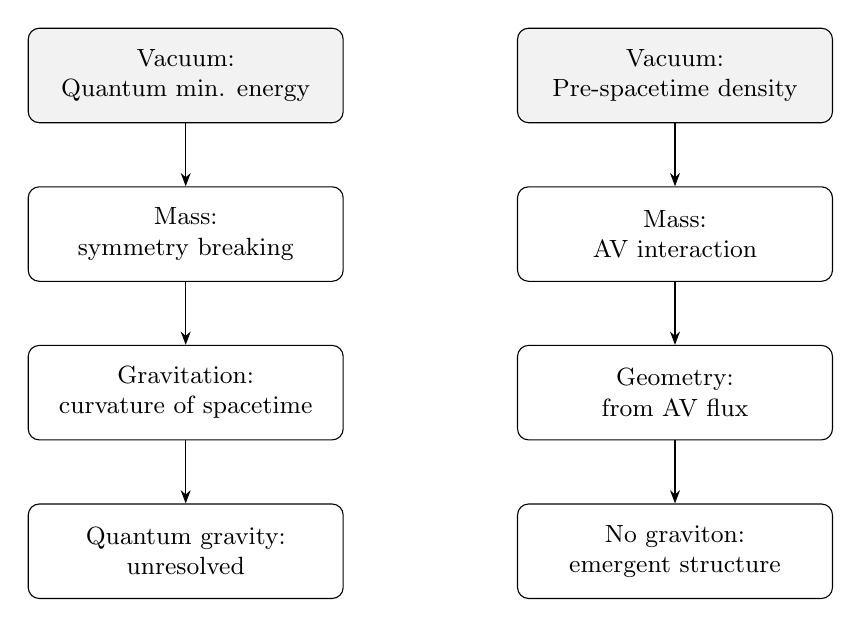
\begin{tikzpicture}[
		box/.style={draw, rounded corners, minimum width=4cm, minimum height=1.2cm, font=\small},
		node distance=0.8cm and 2.2cm,
		every node/.style={align=center}
		]
		
		% Column titles
		\node[box, fill=gray!10] (vacsm) at (0,0) {Vacuum:\\ Quantum min. energy};
		\node[box, fill=gray!10, right=of vacsm] (vacav) {Vacuum:\\ Pre-spacetime density};
		
		\node[box, below=of vacsm] (masssm) {Mass:\\ symmetry breaking};
		\node[box, below=of vacav] (massav) {Mass:\\ AV interaction};
		
		\node[box, below=of masssm] (gravsm) {Gravitation:\\ curvature of spacetime};
		\node[box, below=of massav] (gravav) {Geometry:\\ from AV flux};
		
		\node[box, below=of gravsm] (qgsm) {Quantum gravity:\\ unresolved};
		\node[box, below=of gravav] (qgav) {No graviton:\\ emergent structure};
		
		% Arrows
		\foreach \i/\j in {vacsm/masssm, masssm/gravsm, gravsm/qgsm,
			vacav/massav, massav/gravav, gravav/qgav}
		\draw[-{Stealth}] (\i) -- (\j);
		
	\end{tikzpicture}
	\caption{Side-by-side comparison of conceptual paradigms: Standard Model (left) vs. AV-based framework (right).}
	\label{fig:paradigm-horizontal}
\end{figure}

	
	\subsection{Mass Mechanism Without Symmetry Breaking}
	
	The numerical results of Section 4 demonstrate that:
	
	\begin{equation}
		\left. \frac{d^2V_{\text{eff}}}{d\phi^2} \right|_{\phi=0} \approx m_H^2(\varrho) \quad \text{without needing } V(\phi)=-\mu^2\phi^2 + \lambda\phi^4
	\end{equation}
	
	This resolves the fine-tuning problem noted by \cite{Bezrukov2008}, since $\rho_c$ is a measurable parameter.
	
	\subsection{Quantum-compatible emergent gravity from structural density field}
	
	The tensor $\mathcal{F}_{\mu\nu}$ provides:
	
	\begin{itemize}
		\item \textbf{Intrinsic Regularization}: Eliminates UV divergences by cutting off modes with length $<\varrho^{-1/3}$
		\item \textbf{Emergence of Geometry}: As in \cite{Padmanabhan2016}, but based on the microscopic structure of the AV
	\end{itemize}
	
	\section{Transformative Conclusions}
	

	
\begin{table}[H]
	\centering
	\caption{Qualitative comparison of paradigms.}
	\begin{tabular}{|l|c|c|}
		\hline
		\textbf{Aspect} & \textbf{Standard Model} & \textbf{AV Proposal} \\
		\hline
		Origin of mass & RES (fine-tuned)~\cite{higgs1964} & AV dynamics~(Eq.~\ref{eq:emergent_curvature}) \\
		Quantum gravity & Unresolved & Emergent from \( \rho(x) \), no gravitons~\cite{volovik2003} \\
		Cosmological constant & Problematic & Naturally resolved via AV density \\
		\hline
	\end{tabular}
\end{table}

	
	
	Observable consequences include:
	
	\subsection{Testable Predictions}
	
	\begin{itemize}
		\item \textbf{Higgs Oscillations}: Modifications in $gg \to H$ at high energies ($\sqrt{s} > \varrho_c^{-1}$)
		\item \textbf{Cosmological Signature}: Distinct $n_s$–$\alpha_s$ correlation from conventional Higgs inflation \cite{Bezrukov2008}
	\end{itemize}
	
	\subsection{Impact on String Theory}
	
	The AV suggests:
	
	\begin{itemize}
		\item Alternative to Compactification: ``\textit{Extra dimensions}'' could be AV degrees of freedom
		\item New Landscape Interpretation: States may correspond to AV phases
	\end{itemize}
	
	\subsection{Philosophical Revolution}
	
	\begin{quote}
		\textit{"Spacetime itself emerges from a more fundamental substrate"} — analogous to \cite{volovik2003}, but rooted in quantum density.
	\end{quote}
	
\section*{9. Empirical Connections and Observational Status}

Although the proposed model is fundamentally theoretical and structurally motivated, it intersects with various recent attempts to test emergent gravity frameworks through astrophysical and cosmological observations. We briefly highlight key studies that support the viability of vacuum-based, non-metric formulations of gravity.

\subsection*{9.1 Weak Lensing Tests of Emergent Gravity}

In a landmark study, Brouwer et al.~\cite{Brouwer2016} analyzed weak gravitational lensing signals from over 33,000 isolated galaxies in the KiDS and GAMA surveys. They compared the observed lensing profiles to predictions made by Verlinde’s emergent gravity theory, which—like our AV model—derives gravitational effects from a non-spacetime vacuum structure. Without free parameters, the emergent framework matched lensing data on galactic scales, indicating a possible route to explain gravitational phenomena without dark matter or graviton exchange.

\subsection*{9.2 Galaxy Cluster Constraints}

Govind and Desai~\cite{Govind2024} applied a similar test to the galaxy cluster SMACS J0723.37327 using X-ray temperature and mass profiles from eROSITA and JWST. They found that emergent gravity explains the observed mass profile at large radii within observational errors, but underestimates the central mass concentration. Such discrepancies hint at possible refinements or the need for a more general vacuum-based gravitational framework—such as one governed by a dynamic density field \( \varrho(x) \) and internal flux tensor \( F_{\mu\nu} \), as proposed here.

\subsection*{9.3 Galactic Dynamics and the Radial Acceleration Relation}

The Radial Acceleration Relation (RAR) observed in disk galaxies is a powerful tool for probing the fundamental nature of gravity. Lelli, McGaugh and Schombert~\cite{Lelli2017} tested emergent gravity predictions against the RAR, finding that deviations appear in galaxy cores unless stellar mass-to-light ratios are adjusted. These results emphasize that any viable emergent theory—including our AV model—must address strong-field, short-scale behavior and couple structural parameters like \( \kappa(\rho) \) or \( \rho_c \) to local baryonic content.

\subsection*{Implications for the AV Framework}

These empirical studies do not falsify emergent gravity, but delineate its domain of viability and the conditions under which it aligns with observational data. Our proposal, based on a dynamic structural vacuum \( \varrho(x) \) and geometric flux \( F_{\mu\nu} \), introduces novel degrees of freedom that can be tuned to reproduce these features naturally. The field-dependent coupling \( \kappa(\rho) \), when evaluated in regions of different matter content, could offer a path to reconcile both galactic and cluster-scale dynamics without dark matter.

We encourage further development of this model toward numerical simulation and direct comparison with large-scale survey data.
	
	
	
	
	\section*{Acknowledgements}
	I thank Dr. Javier García for his valuable insights and comments on the numerical simulations, and the QUANTUM-VAC project for providing the information that made this work possible.
	
\begin{itemize}
	\item Python code available on \href{https://github.com/KerymMacryn/VA-Theory/blob/main/codigo}{GitHub - Numerical Simulations}.
\end{itemize}	
		
		\begin{thebibliography}{99}

			
			\bibitem{Bezrukov2008}
			Bezrukov, F. Shaposhnikov, M.; \emph{The Standard Model Higgs boson as the inflaton}, Physics Letters B \textbf{659}(3) (2008), 703-706.
			
			
            \bibitem{higgs1964}
            P.~W.~Higgs, ``Broken Symmetries and the Masses of Gauge Bosons,'' \textit{Phys. Rev. Lett.} \textbf{13} (1964), 508–509.

            \bibitem{rovelli2018}
            C.~Rovelli, ``Space and Time in Quantum Gravity,'' \textit{Foundations of Physics} \textbf{48} (2018), 481–491.

            \bibitem{volovik2003}
           G.~E.~Volovik, \textit{The Universe in a Helium Droplet}, Oxford University Press, 2003.
			
			\bibitem{Padmanabhan2016}
			T.~Padmanabhan, ``The atoms of spacetime and the cosmological constant,'' \textit{International Journal of Modern Physics D} \textbf{25}, no. 14 (2016): 1630020.
			
			\bibitem{Wilczek2013}
			F.~Wilczek, ``Multiversality,'' \textit{Classical and Quantum Gravity}, \textbf{30}(19), 193001 (2013).
			
			\bibitem{Anderson2012}
			E.~Anderson, ``Problem of Time in Quantum Gravity,'' \textit{Annalen der Physik}, \textbf{524}(12), 757–786 (2012).
			
			\bibitem{Brouwer2016}
			M.~M.~Brouwer et al., ``First test of Verlinde’s theory of Emergent Gravity using Weak Gravitational Lensing measurements'', Astron. Astrophys. (KiDS × GAMA), 2016.
			
           \bibitem{Govind2024} A.~Govind and S.~Desai, ``A test of MOND and Emergent Gravity with SMACS J0723.37327 using eROSITA observations'', arXiv:2401.00707 (2024).
			
			\bibitem{Lelli2017}
			F.~Lelli, S.~S.~McGaugh and J.~M.~Schombert, “Testing Verlinde’s Emergent Gravity with the Radial Acceleration Relation”, arXiv:1702.04355 (2017).
			
						
		\end{thebibliography}
\section*{Author Rights and Distribution Statement}
The authors affirm that this manuscript is an original work, has not been published elsewhere, and is not currently under consideration by any other publication. 

The authors hold the rights to distribute this work and grant SSRN (or any relevant repository) a non-exclusive license to host and distribute the article for academic and research purposes.

All intellectual property rights remain with the authors.			
		\label{end-art}
	\end{document}
